The build process is by far the most expensive operation on a k-d tree, and parallelizing it could reduce the overall runtime significantly, when solving the kNN problem. This is not as straight-forward as it might seem. The serial k-d tree build algorithm is usually implemented as a recursive function, since recursive functions tend to go along well with tree-based data structures. On the other hand, performance in CUDA is based on efficient use of a massive number of lightweight threads, and to get a fast algorithm one have to split the work between as many threads as possible. This is only possible if it is easy to divide the work into independent subtasks, where data communication is kept at a minimum. In a recursive context, execution flow in hidden inside each threads call stack. Information needed by other threads is therefore not easy to obtain. To solve this, a iterative approach should be used, which can be implemented with a global accessible execution flow. This will however, give a more complex k-d tree build algorithm, and it is not certain that this algorithm is easy to parallelize. 

\begin{myrq}
\label{rq:parallel_build}
    It is possible to parallelize the k-d tree build algorithm, in such a way that it gives a significant speed improvement compared to the serial algorithm.
\end{myrq}

In order to investigate RQ~\ref{rq:parallel_build}, we have to look a bit closer at the different steps of the k-d tree build algorithm and investigate different parallelization strategies.

\subsection{From recursive to iterative implementation} % (fold)
\label{ssub:from_recursive_to_iterative_implementation}

Before we dive into the parallelization strategy and how the parallelization can be done, lets try to make a iterative solution. We can start by enumerating the different steps in the recursive implementation.

\begin{enumerate}
    \item Find the median of the points along a specified axis. This median point becomes the value of the current node.
    \item Sort all points with lower values than the median to the left of the median, and all the points with higher values than the median to the right.
    \item Perform this algorithm recursively on the left and right set of nodes.
\end{enumerate}

From the steps one can see that for each node in the k-d tree, one have to partition a list around it's median. We will call this operation Balance-Subtree. If we analyze the Algorithm~\ref{alg:seriel_tree_build}, we see that there are two recursive calls. This is logical, because we are building a binary tree where each node have two children. The interesting observation is that a node balance is only dependent on the parent node. This means that each tree level are independent and can be done iteratively.

The k-d tree construction basically boils down to successively balance each node in the tree. This leads to a basic reimplementation, see Algorithm~\ref{alg:iterativ_tree_build}. It goes through each level of the tree, starting at the top, and balances each node successively down the tree.

\begin{algorithm}
\caption{Iterative k-d tree build}
\label{alg:iterativ_tree_build}
\begin{algorithmic}
    \Require{An array of points, $T$}
    \Ensure{$T$, as a k-d formated array}
    \Function{Build-KD-Tree}{$T$}
        \ForAll{$L \in \{\text{all levels in } T\}$}
            \ForAll{$S \in L$}
                \State$d \gets |L| \bmod k$ \Comment{k = 3 for a three dimensional k-d tree}
                \State \Call{Balance-Subtree}{$S$, $d$}
            \EndFor
        \EndFor
    \EndFunction
\end{algorithmic}
\end{algorithm}
% subsection from_recursive_to_iterative_implementation (end)

\subsection{Parallelization strategy} % (fold)
\label{ssub:parallelization_strategy}

Now that an iterative solution have been created, lets start looking at how this algorithm might be parallelized. First a good overall parallelization strategy has to be found. A good strategy manage to easily split the main task into small individual subtasks, that can be performed in parallel, while maintaining a minimal need for communication between the subtasks.

%TODO: One observation. Children in same tree can be done in parallel. Implies one parallelization.
When we converted our k-d tree algorithm from a recursive to a iterative solution two interesting observations was made. The first observation is that a node balance is only dependent on the parent node. This means that each tree level are independent, which acts as a good start for our parallelization strategy.

This also means that all subtrees in the k-d tree generation are independent. Hence, the tree corresponding to the left and right child of a node can be done in parallel without any communication. 

The data is also independent, as a result of how we represent the tree as an array. By data independent, it is meant that the data structure easily can be partitioned to each subtask. In our case will the tree array successively be partitioned into contentious subtrees.

From these observations, several strategies can be used to parallelize the k-d tree build algorithm. The first observation implies that we can divide the tree levels into dependent tasks, where each node balance in a tree level is a independent subtask. This gives us an power of two increasing number of parallel tasks as we go down a tree level. The sublist size will decrease with a factor of two in each downward step, see Fig~\ref{fig:tree_level_development}

This parallelization strategy gives many concurrent operations at the lower level of the tree, but at the initial levels, we hardly get any parallelization at all. To cope with this we can seek to parallelize the work done in each Balance-Subtree procedure.

Both strategies can be used in conjunction with each other. The parallel balance node task algorithm can be used to speed up the early iterations, where the amount of nodes in a tree level is small. As well as further parallelize the subtasks in later tree level iterations. This strategy also fit well to our choice of tree representation. One parallel operation can now take the tree representation, split it into subtrees, and balance each subtree. Everything can also be done in place, so the algorithm is as memory efficient as possible.

\begin{figure}[ht!]
\centering
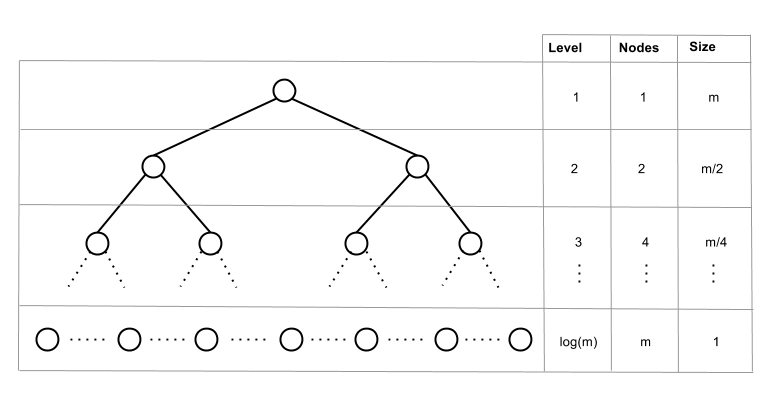
\includegraphics[width=100mm]{../gfx/Tree_level_development.png}

\caption{Development of subtasks as the kd-tree generation progresses. It shows, at each tree level, how many nodes there is to parallelize and how big each node balancing is. }
\label{fig:tree_level_development}
\end{figure}
% subsection parallelization_strategy (end)

\subsubsection{CUDA parallelization} % (fold)
\label{ssub:divide_work_on_cuda}

CUDA have a special architecture that should be taken into account when parallelizing an algorithm. To efficiently use CUDA, the program has to keep thousands of threads occupied, otherwise the benefit of CUDA disappears. The CUDA programming model is build up by a grid if independent block, i.e.\ execution can not be synchronized across blocks. Execution can only be synchronized between the 1 to 1024 theoretical threads launched inside a block~\cite{cuda_programming_guide}. Thread synchronization is important when multiple threads cooperate on one task, because at some point information has to be exchanged.

Our parallelization strategy states that we have to balance one tree level after another, since they are dependent. This implies that the threads need to communicate between each tree level. One CUDA kernel should therefore balance a complete tree level. The other alternative would be to build the hole tree in one block, which would restrict our kernel to only be executed on one SM\@.

The next step is to split the tree level balance between the CUDA resources. The number of node in a tree level increases with the power of two, as we go down the tree. Fig~\ref{fig:tree_level_development} shows that our kernel, the tree balance, changes throughout the build process. First only one node needs to be balanced, e.g only one parallel operation. At the end there are $m$ different nodes to work on. The problem size also changes, at the top, it is $m$ per node and goes towards $1$, as the tree level increases.

This varying problem sizes and subtasks, makes it hard to create a good work distribution between the CUDA resources. At the top part of the tree it is optimal to use many blocks to balance a node, but at the end, it is desirable to balance many nodes inside a block. We choose a middle ground, to balance one node in one block. This means that there should be an overall good performance with a peek at the middle three levels.
% subsection divide_work_on_cuda (end)

\subsection{Parallelization of Subtree-Balance} % (fold)
\label{ssub:selecting_a_algorithm}

With the overall parallelization strategy planned, we can start investigate the most time-consuming operation, balancing a tree level. We have already determent that the parallelization should be done in one block, which means that one operation is done per SM\@. In other words, the task can potentially be parallelized between 1024 theoretical threads. Lets start investigating different approaches.

The main operation is to find a median. As we have seen in Section~\ref{sub:application_of_kd_trees_to_the_knn_problem}, many algorithms for finding median exist. Since we now want to implement the algorithm with CUDA, the environment has changed, and quick-select may not be the best alternative anymore. The first problem with quick-select is that it is recursive, which makes it hard to parallelize on CUDA\@. Therefore it may be profitable to look at other, more parallelization friendly, algorithms.

First reusing the bitonic sort was investigated. Given a sorted list one can find the median directly, by simply looking at the midmost element of the array. The partitioning is also done in the process. Unfortunately this strategy proved unsuccessful, as re-purposing the bitonic algorithm for such an task proved difficult. The reason for this is that a pure bitonic sorting network only manage to sort lists with a length of power of two. The normal solution is to create a longer list then needed, but wasting this much memory on on the GPU is not a very good solution. 

Another way to make bitonic sort work with a list of any size is described by K.E. Batcher~\cite{Batcher:1968}. The description of this solution is very lengthy, and has been omitted, since it introduces a lot of divergence, that would be decremental to performance on the GPU\@. We also have the inherent downside of sorting a list in order to find the median, since \BigO{m} algorithms for finding the median exist, compared to the \BigO{m log(m)} time required by sorting.

%TODO: Check agglomeration vs adversarial
Bucket-sort and radix-sort based algorithms are investigated in the paper Fast K-selection Algorithms for Graphics Processing Units by Alabi et.al\@.~\citep{Alabi:2012}. The big difference between them is the constant time penalty. The radix sort have a more exact time complexity of \BigO{b\ m}, where b is the number of bits in each number. While the penalty for bucket select is \BigO{a\ m}, where $a$ denotes the degree of agglomeration in the values. In other words, the algorithm is week when the points are clusters together. His results shows that bucket select normally is slightly faster, except when $a$ is high. Although bucket select normally have better results, we expect a high degree of agglomeration in our application, so we choose radix select.
% subsubsection selecting_a_algorithm (end)

\subsubsection{Radix select} % (fold)
\label{ssub:radix_select}

The radix select is based on a bitwise partitioning, much like radix sort~\cite[Chapter 8.3]{Cormen:2001}. In each step, elements are partitioned in two subgroups based on the current bit. Then the subgroup that contains the median is determined, and the search continue in that subgroup until the median is found.

\begin{figure}[ht!]
\centering
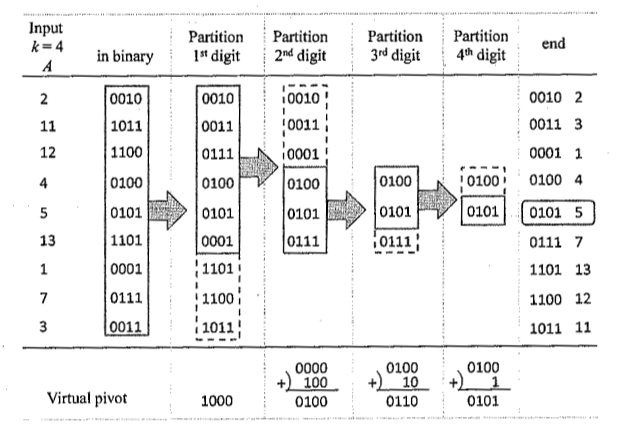
\includegraphics[width=100mm]{../gfx/Radix_select.png}

\caption{An illustration of radix selection~\cite{cayman:2012}.}
\label{fig:radix_select}
\end{figure}

When it comes to create a parallelization strategy for radix select it is first advisable to take a look at a highly optimized radix sort, like the variant introduced by Merrill~\cite{MerrillG11}. The radix select can easily be reduced from a radix sort, and many concepts can therefore be reused. An other interesting implementation is the radix select by Alabi~\citep{Alabi:2012}. They both uses a parallelization strategy by splitting each radix partition into parallel operations. The way our and Alabi's solution differs from Merrill's solution, is that we start on the most significant digit, since a least significant digit approach will not reduce the k'th order statistic problem in each step.
% subsection radix_select (end)

\subsubsection{Our implementation} % (fold)
\label{ssub:our_implementation}

% TODO: Ta med bigO kalkulasjon på hele algorithmen.
Our implementation is based on Algorithm~\ref{alg:iterativ_tree_build}. Calling Balance-Subtree on all nodes in a tree-level, is performed on the GPU as a CUDA kernel. The outer for-loop is executed on the CPU, and launches the kernel for increasing tree-levels, until the entire tree is built. The complete implementation can be found in Appendix~\ref{sec:paralell_k_d_tree_build}.

Algorithm~\ref{alg:parallel_balance_subtree} is parallelized only within a single CUDA block. This means that the parallel threads are able to communicate. The algorithm is based around a repeat-until loop, which basically do all the work. The loop keeps track of a partition array. This array is then sliced in to, by giving each thread a portion of the array, each thread then counts how many zeros it finds in the current bit position. The cut, as the arrows in Figure~\ref{fig:radix_select} shows, is calculated by doing a reduce sum operation~\citep{parallel_reduction_in_cuda}. This is repeated until the partition contains the median, which is when every bit is used or when the partition size is one. After the loop, the array is transformed. Such that the median is in the center, with lesser elements on the left and bigger on the right.

\begin{algorithm}[ht]
\caption{Parallel subtree balance}
\label{alg:parallel_balance_subtree}
\begin{algorithmic}
    \Require{A subtree $S$ of length $m$, and dimension $d$}
    \Ensure{A balanced subtree, $S$}
    \Function{Balance-Subtree}{$T$, $d$}
        \State Let $l$ and $u$ be the upper and lower bond of current partition.
        \State Let $P$ be all nodes in $S$
        \Repeat
            \ForAll {$\{p \in P \mid l < p < u\}$}
                \State $Z(t) \gets $  \text{Occurrences of zeros in current bit, $b$, found by thread, $t$.}
            \EndFor
            \State $c \gets \Call{Sum-Reduce}{Z}$ \Comment{$c$ is the cut of the current partition $P$.}
            \If{$u-c \ge m/2$}
                \State$ u \gets u-c$
            \Else
                \State$l \gets u-c$
            \EndIf
            \State $b \gets b+1$ \Comment{Move to the next bit}
            \State \Call{Synchronize-Threads}{\ }
        \Until{$u-l<1 \lor b > \Call{Radix}{p \in P} $}
        \State \Call{Partition}{$S, P$}
    \EndFunction
\end{algorithmic}
\end{algorithm}

In CUDA thread instruction run sequentially in warps of 32. Control flow divergence within a warp can therefore significantly destroy the instruction throughput. This is because the different execution paths must be serialized, as all the thread in a warp share the same program counter~\cite{cuda_c_best_practices_guide}. The total number of instruction in a warp will therefore increase. Any conditional operator, e.g\@. if and switch, should be used with care, since it may branch the control flow. Optimizing the use of conditionals, in order to reduce the amount of branching in the program control flow, will give better performance.

In our implementation, all threads perform the same thing in every iteration. This will give a low thread branching. The loop is also almost done equal times by all thread, one time for each bit used to represent the points. The one $if$ statement in the iteration, can be reduced to only contain one statement, which make the divergent thread branch small. The code is therefore good in regard of divergence.

An other aspect to consider, is the CUDA memory hierarchy. It is beneficial to use the fastest suitable memory. In our case, this include the shared memory, which is a fast memory shared between all threads in a block. The downside is the memory size, it may not be enough space to store our subtree. Although we may not be able to store the hole subtree, there are some date we can put in the shared memory. The zero counter array, shown as $Z(t)$ in Algorithm~\ref{alg:parallel_balance_subtree}, is a perfect candidate. Every thread only use one integer and it is shared between all threads throughout the execution. It will therefore cause a big impoverishment.

The complete implementation can be found in Appendix~\ref{sec:multiple_radix_select}.
% subsection our_implementation (end)

\subsection{Further improvements} % (fold)
\label{ssub:further_development}

Let us take a step back and look at RQ~\ref{rq:parallel_build}. The possibility of parallelizing the build algorithm is achieved. Initial optimization has been performed, so according to the APOD design cycle, we should test our implementation.

\begin{figure}[ht!]
\centering
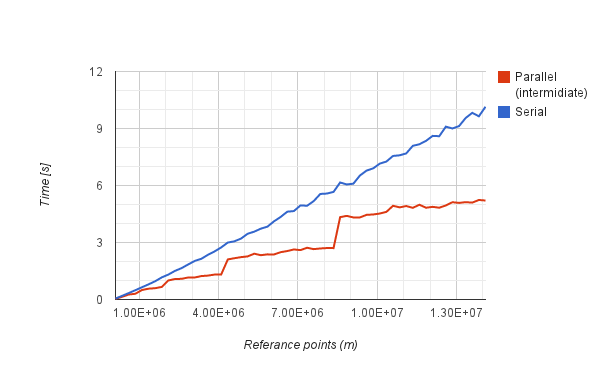
\includegraphics[width=100mm]{../gfx/the_jumps.png}

\caption{Timing results from a intermediate version of the parallel k-d tree build algorithm.}
\label{fig:gpuv1_vs_cpu}
\end{figure}

With the test setup as described in Section~\ref{sec:test_environment}, the current version of the algorithm gave results as shown in Figure~\ref{fig:gpuv1_vs_cpu}. The most interesting observation are the big jumps in the graph. If one look closely these jumps happens every time the problem size exceeds a power of two, as for example when the size passes $8388608$ the timing increases from $2703 ms$ to $4335 ms$. The results of further investigation is shown in Table~\ref{tbl:nvprc_balance_branch}. It shows how long time each tree level takes, and how the different tree level operations varies throughout the build process.

\begin{table}[ht]
\centering
    \begin{tabular}{|l|l|l|l|}
        \hline
        \textbf{Tree level} & \textbf{Time [ms]} & \textbf{Subtrees} & \textbf{Size}\\ \hline
        1          & 52       & 1                  & 1000000      \\ \hline
        2          & 26       & 2                  & 500000       \\ \hline
        3          & 13       & 4                  & 250000       \\ \hline
        4          & 8        & 8                  & 125000       \\ \hline
        5          & 7        & 16                 & 62500        \\ \hline
        6          & 6        & 32                 & 31250        \\ \hline
        7          & 6        & 64                 & 15625        \\ \hline
        8          & 6        & 128                & 7812         \\ \hline
        9          & 7        & 256                & 3906         \\ \hline
        10         & 7        & 512                & 1953         \\ \hline
        11         & 8        & 1024               & 976          \\ \hline
        12         & 10       & 2048               & 488          \\ \hline
        13         & 16       & 4096               & 244          \\ \hline
        14         & 26       & 8192               & 122          \\ \hline
        15         & 52       & 16384              & 61           \\ \hline
        16         & 105      & 32768              & 30           \\ \hline
        17         & 202      & 65536              & 15           \\ \hline
        18         & 389      & 131072             & 7            \\ \hline
        19         & 768      & 262144             & 3            \\ \hline
    \end{tabular}
    \caption{Development of a k-d tree build with a million points, showing how the different tree level operations varies throughout the build process.}
    \label{tbl:nvprc_balance_branch}
\end{table}

The table reveal some weaknesses of our algorithm, that is based around how the CUDA resources was divided in Section~\ref{ssub:divide_work_on_cuda}. It performs badly when the problem size or the number of subtrees is relatively large. The potential for parallelizing the workload for the first and last iterations is not being fully utilized. This is due to the implementation forcing one version of the radix select algorithm to work on all problem types. This is not optimal for dividing CUDA resources, and as a result, we get high penalties when the problem reaches unsuitable values.

This hypothesis can also explain the big jumps in runtime. The observations above correlates perfectly with the tree hight, since the hight of a binary tree is the binary logarithm of the tree size. This implies that the jumps happens when an additional tree-level is required in order to fit the tree.

Tuning the algorithm to alternate between different algorithms to balance a subtree, eliminates this problem. This removes the penalty for calculating the median at unsuitable problem sizes.

Our current implementation only use one block per subtree, which means we are only able to use one SM to balance the subtree. By utilizing several blocks at the same time, big subtrees could be processed faster. However, since all blocks are used to balance one subtree, only one subtree can be balanced at a time.

The implementation details are omitted here, but can be found in Appendix~\ref{sec:radix_select}. In short, the implementation follows the outline of the radix-select implementation, but the thread synchronization is performed on the CPU, between kernel launches. This enables us to communicate between the different blocks.

We also would like to improve performance, when Balance-Subtree is applied to many small subtrees. For instance, at level $18$ there are $131072$ different subtask with only an average size of $7$. The previous implementation divided all these subtask between a small number of SM, typically $8-32$ on current NVIDIA GPUs\@. The algorithm the uses to many cores to balance a subtree of only $7$ elements, which is not a efficient way to divide resources.

Letting just one thread handle the Balance-Subtree operation for small subtrees, would let us process more subtrees in parallel, improving performance. With this parallelization, each thread is responsible for it's own subtree, and communication with other threads is no longer needed. With the need for communication eliminated, we can utilize Algorithm~\ref{alg:seriel_tree_build}. 

\begin{figure}[ht!]
\centering
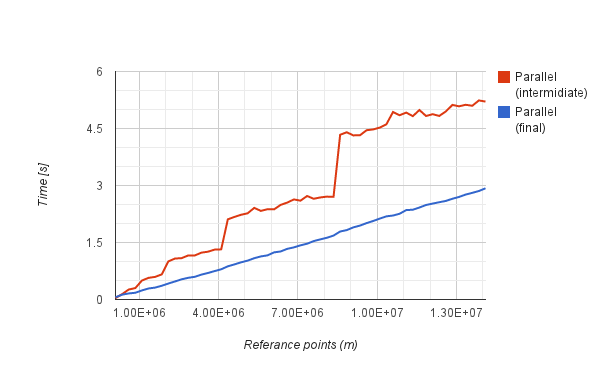
\includegraphics[width=100mm]{../gfx/the_jumps_final.png}
\caption{Visualization of the final improvments on the k-d tree build implementation.}
\label{fig:the_jumps_final}
\end{figure}

Now that a lot of improvements have been made, lets take a look at the results. Figure~\ref{fig:the_jumps_final} compare our intermediate result with our new and improved version, and the changes made a huge impact on the performance. The jumps disappeared, and was replaced by a faster and smoother curve, indicating that the CUDA resources is perfectly balanced. The final implementation can be found in Appendix~\ref{sec:parallel_quick_select}.
% subsection further_development (end)
